\chapter{String Processing}

\section{Regular Expressions}

\subsection{Regular Expressions}

\subsection{Zero-width Lookahead Technique}

\begin{figure}
    \centering
    % Wikipedia Public Domain image
    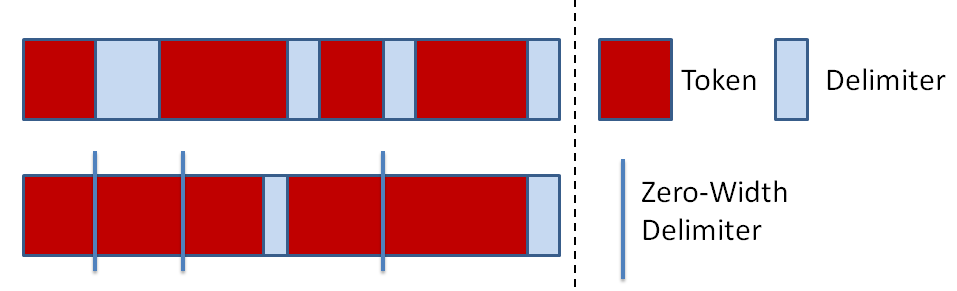
\includegraphics[height=1.5in]{lookaheadsplitting.png}
    \caption{Lookahead Splitting}
    \label{fig:lookaheadsplit}
\end{figure}

\subsection{NFA Simulation}
\index{NFA!Simulation}

The Regex engine in Java does not convert to a Thompson-DFA; it uses a backtracking algorithm
to find out if a regular expression matches a string.  This leads to pathological cases with
exponential runtime increase, particularly when the regular expression contains a large number
of Kleene stars.

In those situations, it may be helpful to construct your own mini-regexp interpreter by building
and simulating an NFA (nondeterministic finite automaton).

Example problem is \href{http://ncpc.idi.ntnu.no/ncpc2011/ncpc2011problems.pdf}{NCPC 2011/E}
where the input are globs such as \texttt{*a*a*a*a} that should be matched against filenames.

\inputminted{python}{code/ls.py}

\section{Parsing}
\subsection{Recursive Descent}

